\PassOptionsToPackage{unicode=true}{hyperref} % options for packages loaded elsewhere
\PassOptionsToPackage{hyphens}{url}
%
\documentclass[]{memoir}
\renewcommand\cftappendixname{\appendixname~}
\usepackage{lmodern}
\usepackage{geometry}
\usepackage{amssymb,amsmath}
\usepackage{upgreek}
\usepackage{ifxetex,ifluatex}
\usepackage{fixltx2e} % provides \textsubscript
\usepackage{hyperref}
\usepackage{mdframed} % gives figure color bg
\usepackage{url}
\usepackage{graphicx,grffile}
\usepackage{tabularx}
\usepackage{threeparttable}
\usepackage{lscape}
\usepackage{booktabs, multirow} % for borders and merged ranges
\usepackage{soul}% for underlines
\usepackage[table]{xcolor} % for cell colors
\usepackage{changepage,threeparttable} % for wide tables
\usepackage[backend=bibtex,giveninits,style=numeric,sorting=none]{biblatex}
\addbibresource{../biblio.bib}
%\usepackage{cite}
\usepackage{longtable}
\usepackage{paralist}
\usepackage{rotating}
\usepackage{ltxtable}
\usepackage{import}
\usepackage{caption}
\usepackage[para]{footmisc}
%\usepackage{fancyref}
\usepackage{acro}
\usepackage{bm}
\usepackage{afterpage}
\usepackage[section]{placeins}
\usepackage{appendix}
\usepackage{enumitem}
%\usepackage[backend=bibtex,giveinits,style=unsrt]{biblatex}


% probably a good idea for the nomenclature entries:
\acsetup{first-style=short}


\ifnum 0\ifxetex 1\fi\ifluatex 1\fi=0 % if pdftex
\usepackage[T1]{fontenc}
\usepackage[utf8]{inputenc}
\usepackage{textcomp} % provides euro and other symbols
\else % if luatex or xelatex
\usepackage{unicode-math}
\defaultfontfeatures{Ligatures=TeX,Scale=MatchLowercase}
\fi

% use upquote if available, for straight quotes in verbatim environments
\IfFileExists{upquote.sty}{\usepackage{upquote}}{}
% use microtype if available
\IfFileExists{microtype.sty}{%
	
	\usepackage[]{microtype}
	\UseMicrotypeSet[protrusion]{basicmath} % disable protrusion for tt fonts
}{}

\IfFileExists{parskip.sty}{%
	\usepackage{parskip}
}{% else
	\setlength{\parindent}{0pt}
	\setlength{\parskip}{6pt plus 2pt minus 1pt}
}

\hypersetup{
	pdfborder={0 0 0},
	breaklinks=true}
\urlstyle{same}  % don't use monospace font for urls
\setlength{\emergencystretch}{3em}  % prevent overfull lines
\providecommand{\tightlist}{%
	\setlength{\itemsep}{0pt}\setlength{\parskip}{0pt}}
\setcounter{secnumdepth}{0}
% Redefines (sub)paragraphs to behave more like sections
\ifx\paragraph\undefined\else
\let\oldparagraph\paragraph
\renewcommand{\paragraph}[1]{\oldparagraph{#1}\mbox{}}
\fi
\ifx\subparagraph\undefined\else
\let\oldsubparagraph\subparagraph
\renewcommand{\subparagraph}[1]{\oldsubparagraph{#1}\mbox{}}
\fi






% set default figure placement to htbp
\makeatletter
\def\fps@figure{htbp}
\makeatother

\newcommand{\todo}[1]{{\textcolor{red}{\textbf{#1}}}}

\newcommand{\pplfont}[1]{{\fontfamily{ppl}\selectfont #1}}

\newcommand{\lmttfont}[1]{{\fontfamily{lmtt}\selectfont #1}}

\setcounter{tocdepth}{3}
\setcounter{secnumdepth}{3}

%\title{New radiomics approaches for hepatic tumor characterization by imaging analysis}

%\author{OUHMICH Farid\\{\small Supervised by: AGNUS Vincent, HEITZ Fabrice \& NOBLET Vincent}}


\renewcommand{\baselinestretch}{1.75}

\renewcommand{\arraystretch}{5}

\newgeometry{vmargin={15mm}, hmargin={30mm,30mm}}   % set the margins 
\usepackage{tocloft}

\begin{document}


\section{Contexte Scientifique}

\subsection{Radial}

Cette thèse s’inscrit dans le projet Radial mené par l'institut de recherche de chirurgie guidée par l’image à Strasbourg dont l’un des buts est l’amélioration du traitement et de la prévention du cancer du foie.

\subsection{Cancer}

Le cancer est la seconde cause de mortalité au monde et le cancer du foie est le second type
de cancer le plus répandu avec près de 800.000 morts dénombrés en 2019 selon l’OMS.
Les cancers du foie peuvent être caractérisés comme “primaires” avec une apparition et une croissance qui se fait entièrement dans le foie, ou “secondaires”, dans le cas d’une migration de cellules tumorales à partir d’un organe distant, jusqu’au foie pour donner lieu à une tumeur hépatique. 
Bien que moins fréquentes que les tumeurs secondaires, notre travail de recherche portera principalement sur les tumeurs primaires, avec une attention particulière sur les hépatocarcinomes cellulaires (HCC). Cette décision fut prise dans l’optique de préparer une future collaboration avec le professeur Patrick Baumert, expert dans l’étude des HCCs.
De manière générale, la méthode standard pour évaluer la nature d’une tumeur consiste soit à effectuer une biopsie suivie d’une analyse anatomo-pathologique sur les tissus prélevés, soit à acquérir puis analyser des images tomographiques des organes atteints par la maladie. 


\subsection{Biopsie \& Anatomopathologie}

La biopsie, geste invasif, peut être compliquée, voire impossible à réaliser en raison des
difficultés d’accès à la tumeur.
L’anatomo-pathologie est la spécialité médicale dédiée à l’étude morphologique des anomalies macroscopiques et microscopiques des tissus biologiques et des cellules pathologiques prélevés sur un être vivant ou décédé. Elle est cruciale dans la caractérisation des tumeurs par analyse de tissus biopsiés. Classiquement cela implique une analyse visuelle par un médecin anatomo-pathologiste d’un échantillon de tissu prélevé sur le patient, à l’aide d’un microscope, pour identifier leurs propriétés structurales. Actuellement, l’analyse visuelle est un processus très coûteux en temps humain et l’exactitude du diagnostic repose sur la formation et l’expérience personnelle de l’anatomo-pathologiste. Certains standards sont définis internationalement, tels que la classification des tumeurs. Cela permet d’assurer une certaine cohérence entre les observateurs. Cependant, bien que la formation des anatomo-pathologistes et le contrôle de qualité aient abouti à une concordance suffisante dans de nombreux domaines de l’anatomo-pathologie, il existe encore d’importantes variations dans l’interprétation des phénomènes biologiques observés et la précision varie considérablement pour certains systèmes de notation ou biomarqueurs.
Concernant les HCCs, l’analyse anatomo-pathologique donne lieu à une évaluation des tissus prélevés où différentes caractéristiques sont décrites, notamment l’état des cellules hépatiques via un score appelé “grade histologique”. Deux standards existent pour cela, la classification d’Edmonson-Steiner de 1954 et la classification de l’OMS datant de 2010, dont les caractéristiques des différents groupes sont détaillés sur la figure \ref{fig:martins2017_table1}.
\begin{figure}
\centering
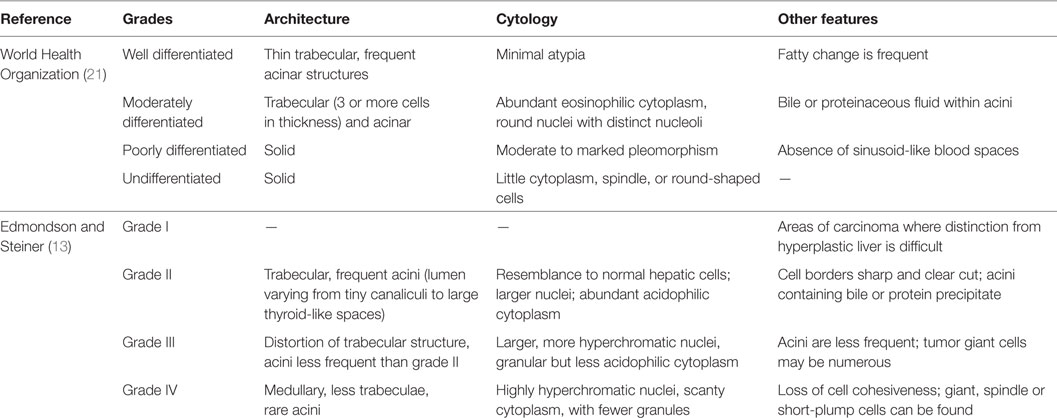
\includegraphics[width=0.7\linewidth]{../HistologicalGradePrediction/images/martins2017_table1}
\label{fig:martins2017_table1}
\end{figure}


\subsection{Hétérogénéité des cancers}
Les cancers présentent une forte hétérogénéité intra et inter-patiente, qui se traduit à différents niveaux : gènes, protéines, cellules, microenvironnement, tissus et organes. Une telle hétérogénéité tumorale limite l’efficacité de la biopsie, car il est peu probable qu’un petit échantillon de tissu soit représentatif de la tumeur globale.
Un exemple d’hétérogénéité présente sur des lames histologiques extraites de tissus hépatiques tumoraux peut être observé sur la figure \ref{fig:pawlik_fig4}.

\begin{figure}
\centering
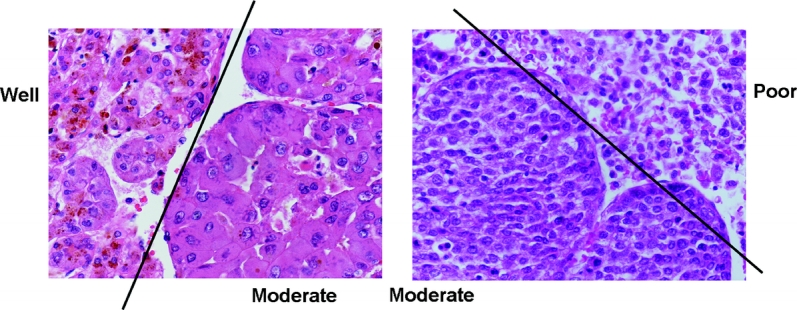
\includegraphics[width=0.7\linewidth]{../HistologicalGradePrediction/images/pawlik_fig4}
\label{fig:pawlik_fig4}
\end{figure}

Une alternative sérieuse à la biopsie consiste en l’analyse, par un expert en radiologie, d’images médicales des zones touchées par la maladie. Cette méthode repose cependant grandement sur l’expertise de l’observateur et souffre également d’une grande variabilité dans les conclusions d’un expert à un autre. 
Notre travail de thèse consiste à proposer des solutions pour permettre une meilleure appréhension des images médicales en utilisant notamment le concept de radiomique.
  
\subsection{Radiomique}

Récemment, les progrès en imagerie médicale et en science des données ont permis l’élaboration d’une nouvelle génération de méthodes d’analyse d’image dites radiomiques \cite{Lambin2012}. Elles reposent sur l’extraction à haut débit d’une grande quantité (>400) de descripteurs quantitatifs \cite{Kumar2012} à partir d’images médicales d’une modalité donnée (par exemple scanner, IRM ou PET), avec pour objectif de fournir une caractérisation du phénotype tumoral (nature, degré de gravité). Une représentation de l’approche est illustrée sur la figure \ref{fig:radiomic}. La radiomique peut fournir des informations complémentaires, interchangeables par rapport à d’autres sources (par exemple la démographie, la pathologie, les biomarqueurs sanguins ou génomiques), en améliorant la sélection individualisée du traitement et la surveillance des patients. La radiomique peut avoir un impact clinique important, puisque l’imagerie est couramment utilisée dans la pratique clinique dans le monde entier, offrant une occasion sans précédent d’améliorer l’aide à la décision à faible coût. 

\begin{figure}
\centering
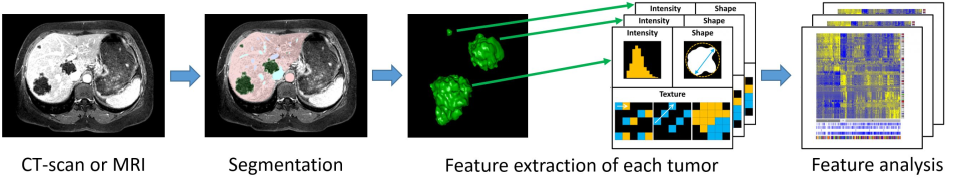
\includegraphics[width=0.7\linewidth]{images/radiomic}
\caption{Workflow d’un projet radiomique : 1) Acquisition d’image, 2) Segmentation par un expert, 3) Extraction automatique des descripteurs, 4) Comparaison à la base d’apprentissage}
\label{fig:radiomic}
\end{figure}


\subsection{Rappel objectif thèse}
L’objectif de cette thèse est de développer de nouvelles approches radiomiques pour la caractérisation des tumeurs hépatiques en analysant et en exploitant la spécificité des images de diagnostics produites. Nous avons décidé d’analyser des images CT pour effectuer la caractérisation des HCCs. De plus, nous nous sommes concentrés sur l’analyse d’images dites “dynamiques” (obtenues à différents moments après injection intraveineuse d’un produit de contraste) afin d’extraire des caractéristiques images liées à des phénomènes cliniques comme le wash-in/wash-out.
L’étude porte sur une base de données contenant les images associées à une analyse phénotypique des tumeurs visibles et segmentées par un radiologue dans chaque image.
Notre algorithme permet de fournir une délinéation précise de la tumeur sur des images dynamiques recalées par le biais d’une architecture de segmentation en cascade, puis d’en extraire des caractéristiques qui seront utilisées pour la prédiction du grade histologique.  


\section{Historique analyse d’images médicales}
Comme évoqué auparavant, l’imagerie médicale apporte une alternative sérieuse à des méthodes invasives telles que les biopsies.
Les récentes améliorations dans le domaine de l’imagerie médicale permettent d’acquérir des données de plus en plus pertinentes pour permettre une meilleure estimation des caractéristiques phénotypiques du patient.
Dans le cas par exemple du cerveau, l’augmentation de contraste, sur des images IRM, rendue possible via l’injection d’un produit de contraste comme le gadolinium est une technique importante pour l’évaluation des tumeurs cérébrales [3, 4]. Cet outil permet une délinéation des grosses tumeurs et une détection précoce des petites lésions métastatiques. Les différentes séquences IRM (comme la carte T1 pondérée) permettent également une séparation des différents tissus au sein d’une même tumeur (tumeur active/nécrose) [3].
Le bénéfice quant à l’utilisation des nouvelles techniques d’imagerie a également été démontré sur d’autres organes comme le foie [5], le sein [6] ou encore le colon [7] avec un apport conséquent en termes de diagnostic.
Cependant, même si l’amélioration des techniques d’imagerie a permis de telles avancées, l’interprétation des images reste le plus souvent subjective et non quantitative. Une telle quantification est possible via l’extraction et l’utilisation de caractéristiques précédemment difficiles voire impossibles à distinguer à l'œil nu.
Les outils d’aide au diagnostic médical (CAD) ont été les premiers, dès les années 80, à tenter d’établir un lien entre les descripteurs “images” et les caractéristiques biologiques du patient [8].
Afin d’accompagner ces nouveaux systèmes, des standards ont vu le jour comme le “WHO” ou le “RECIST” [9] dont l’objectif est d’évaluer l’évolution de la maladie en suivant la progression de la taille de la tumeur, mais encore une fois, ces critères souffrent d’une dépendance trop importante par rapport à l’observateur.
La radiomique à proprement parler a fait son apparition en 2010, permettant de calculer plus de descripteurs que les CADs (plus de 1000 contre seulement 8 à 20 précédemment) et apportant un diagnostic plus complet, les CADs étant la plupart du temps limités à distinguer les masses malignes des masses bénignes [10]. 
Cette nouvelle technique a permis une avancée dans de nombreuses applications que sont le diagnostic du cancer, la détection des tumeurs (avec l’identification des tumeurs malignes), leur classification, l’estimation de la survie du patient, la prédiction de l’agressivité des tumeurs, de la récurrence ou encore du grade de la maladie.
Sur un plan pratique, cette nouvelle technique a également permis d’améliorer l’appréhension des biopsies, en identifiant des zones à risque sur lesquelles effectuer le prélèvement [11], ou bien encore en préconisant de réeffectuer une biopsie [12].
Suite à l’essor du machine et du deep-learning, la radiomique a connu de nombreuses modifications, si bien que deux approches existent à ce jour.
On distingue le paradigme classique (hand-crafted radiomics) qui se base sur des descripteurs dits manuels, de celui où une ou plusieurs étapes font appel à l’apprentissage profond (deep-learning radiomics).

\subsection{Radiomique classique}
L’approche classique nécessite d’effectuer une segmentation manuelle, et de ce fait, sensible à la variabilité inter-observateur [13]. Pour échapper à cette contrainte, des techniques de segmentation semi-automatique ont été mises en place. Certaines, basées sur l’intensité des pixels afin de déterminer leur classe d’appartenance, souffrent du fait que l’intensité des pixels de la tumeur est souvent proche de celle de certains organes avoisinant, d’autres, font appel à des modèles statistiques, nécessitant parfois de calculer une fonction d’énergie trop coûteuse en termes de nombre de paramètres.
Une fois le volume d’intérêt délimité, les différents descripteurs peuvent être extraits. Là encore, deux procédés diffèrent l’un de l’autre. Dans un premier temps, les descripteurs peuvent être choisis a priori pour leur capacité à illustrer le comportement attendu par les experts. C’est le cas par exemple sur le poumon où différentes études ont prouvé une corrélation entre l’homogénéité au niveau textural et le taux de survie [17, 18], ou le grade [16]. Ces connaissances a priori peuvent également être utilisées dans le cas de tumeurs cérébrales pour observer la réaction provoquée par un traitement donné notamment en observant la densité vasculaire et cellulaire [20, 4]. Les connaissances a priori ne sont pas toujours suffisantes pour répondre à un problème donné, c’est pourquoi une autre possibilité est d’extraire une grande quantité de descripteurs et de déterminer les plus pertinents en utilisant par exemple des algorithmes d’apprentissage automatique.
Les descripteurs extraits peuvent être regroupés en différentes catégories : les descripteurs statistiques du premier ordre, ceux du second ordre, et ceux d’un ordre supérieur. Pour les descripteurs de premier ordre, le volume d’intérêt est transformé en histogramme à partir duquel sont calculées différentes valeurs comme l’uniformité ou l’entropie. Ces valeurs étant le plus souvent sensibles aux paramètres d’acquisition de l’image comme l’épaisseur des coupes ou encore les modalités de construction de l’histogramme, ont pourtant permis de déterminer le caractère malin de tumeurs du sein [18].
Des descripteurs de forme peuvent également être directement extraits du volume d’intérêt, afin d’analyser la structure géométrique de ce dernier (comme la surface totale occupée par la tumeur ou encore sa sphéricité). Ces descripteurs ont déjà permis de prédire la réponse provoquée par un traitement [19].
Les descripteurs du second ordre ont comme vocation d’extraire les caractéristiques texturales du volume, en considérant la relation de voisinage entre les pixels, qui joue un rôle important notamment pour la caractérisation de l’hétérogénéité des tissus. Cette relation est capturée par différentes matrices descriptives (GLCM, GLRLM, . . .) [18].
Enfin, les descripteurs d’ordre supérieur permettent de capturer des caractéristiques images dans de nombreux domaines de fréquence (la transformée en ondelette étant la plus fréquemment utilisée [19]).
Un grand nombre de descripteurs peuvent alors être extraits, cependant la plupart d’entre eux sont fortement corrélés, ce qui peut engendrer un sur-apprentissage lors de la création du modèle prédictif. Une phase de réduction du nombre de descripteurs doit alors être effectuée, de manière supervisée (ce qui signifie qu’ils sont sélectionnés en fonction de leur caractère prédictif au regard de la tâche souhaitée), ou non supervisée (le principal objectif étant de supprimer les descripteurs redondants en ne considérant pas les différentes étiquettes) [18].
Parmi les méthodes supervisées, on distingue les méthodes univariées, où les descripteurs sont testés les uns après les autres en fonction de leur contribution à la classe cible (test de Wilcoxon, ou de Fisher), des méthodes multivariées (où les descripteurs sont regroupés dans des sous-ensembles avant de tester leur corrélation avec la classe d’arrivée).
Les méthodes non supervisées (comme l’ACP par exemple) sont quant à elles moins sujettes au sur-apprentissage car elles ne considèrent pas l’étiquette des données, mais n’ont pour seul but que de réduire la dimensionnalité de l’espace des descripteurs.
Une fois le nombre de descripteurs réduit, il reste à construire un modèle prédictif, en utilisant des méthodes de clustering (les patients sont regroupés en fonction d’une métrique dépendante des descripteurs retenus) ou de classification (où des modèles comme les forêts d’arbres aléatoires ou encore les machines à vecteur de support sont entraînés à partir des descripteurs retenus dans le but de prédire le caractère clinique souhaité). Pour la prédiction de la survie du patient, il est commun de faire appel à des modèles un peu différents (Kaplan-meier ou encore Cox Proportional Hazards [20]).
Un des objectifs recherché est la stabilité des descripteurs vis-à-vis des étapes de pré-traitement. Pour cela, le patient peut subir l’examen d’imagerie à plusieurs reprises (test-retest) et les segmentations peuvent être effectuées par plusieurs experts [21].
Une étude radiomique classique repose donc sur la meilleure combinaison entre l’extraction des descripteurs, la technique de réduction ainsi que la méthode de création du modèle.
La moindre modification sur chacune de ces étapes peut avoir un impact conséquent sur le caractère prédictif du modèle résultant, c’est pourquoi une nouvelle branche de la radiomique, se basant en partie ou entièrement sur l’apprentissage profond, a fait son apparition.

\subsection{Radiomique sur base d’apprentissage profond}
Dans cette branche de la radiomique, les descripteurs ne sont plus manuellement extraits, mais ils le sont par le biais de l’apprentissage profond.
Un réseau neuronal profond peut être choisi pour discriminer les descripteurs les plus pertinents, ils peuvent ensuite être conservés dans le réseau afin d’être entraînés sur la tâche souhaitée ou bien être utilisés comme entrée dans un modèle différent (SVM ou arbre de décision par exemple).
Comparé à la radiomique classique, aucune connaissance a priori n’est nécessaire, et les descripteurs peuvent être extraits de manière automatique. Les réseaux profonds peuvent être entraînés de bout en bout, en utilisant uniquement les images originales en entrées, sans nécessairement devoir fournir de segmentation. Il a également été démontré que les performances de ces réseaux allaient en s’améliorant avec un nombre grandissant de données d’entraînement [22].
L’élimination de l’étape de segmentation, lors de la phase d’évaluation du diagnostic, permet de réduire la charge de travail des experts et répond au problème de la dépendance à l’observateur. Les segmentations automatiques n’étaient à ce jour, pas encore suffisamment précises pour pouvoir être utilisées lors d’applications dites “sensibles”.
Lors de l’entraînement, les annotations des différents zones d’intérêt peuvent néanmoins être combinées à l’image originale (de même que d’autres représentations, comme le gradient par exemple [23]) afin d’améliorer la qualité des descripteurs extraits.
D’une manière générale, les études radiomiques faisant appel à l’apprentissage profond peuvent être différenciées selon plusieurs aspects que sont le type d’entrée utilisée, la stratégie d’entraînement et enfin le choix de l’architecture privilégiée pour extraire les descripteurs.
En entrée des réseaux profonds, on peut considérer les coupes 2D indépendamment les unes des autres, cependant cette technique n’apporte pas suffisamment d’information tant la décision dépend grandement de l’intégralité du volume d’intérêt.
Les résultats obtenus coupe à coupe peuvent alors être fusionnés pour obtenir une décision à l’échelle du volume. Ce dernier peut aussi directement être utilisé comme entrée, cependant le problème se pose sur les différences en termes de représentation des volumes (taille des voxels, épaisseur des coupes). Enfin, la classification peut se faire en considérant une série d’études pour le même patient [24], mais là encore un problème de normalisation se pose, tant le nombre de coupes par patient peut varier.
Une fois le type d’entrée choisi, les études peuvent varier en fonction de leur stratégie d’entraînement. Les réseaux peuvent être entraînés entièrement à partir des données à disposition, ou des architectures pré-existantes peuvent être ré-utilisées.
Dans le premier cas, le réseau obtenu sera complètement ajusté à la tâche souhaitée, mais cette spécialisation peut être à l’origine de problèmes comme le sur-apprentissage ou la sensibilité à un déséquilibre de répartition des classes.
L’impact de ces deux problématiques peut être limité à l’aide de l’augmentation de données (utilisation des données d’entraînement existantes pour en générer aléatoirement des nouvelles) [13], l’entraînement multi-tâche (où le nombre de paramètres libres du réseau est limité suite à un entraînement simultané de la même architecture sur des tâches différentes) [25], ou encore l’adaptation de la fonction de coût à la proportion des données de chaque classe [25].
L’autre stratégie consiste à utiliser une architecture pré-entraînée sur des images naturelles la plupart du temps, puis d’en ré-entraîner uniquement une partie sur la tâche souhaitée [29, 30, 31].
Enfin, les différents descripteurs sont extraits, là encore en suivant une approche supervisée ou non-supervisée.
Dans le premier cas, les architectures les plus utilisées sont les réseaux à base de couches de convolution (CNN) avec une ou plusieurs couches denses dont l’objectif est de prédire la classe de sortie. Tandis que le réseau est entraîné à effectuer la classification, les descripteurs sont extraits soit en queue de réseau (après l’une des dernières couches denses) [28], soit après l’une des couches de convolution [29].
D’autres variantes, toujours à base de couches de convolution, ont vu le jour, comme le RNN (recurrent neural network), le LSTM (long-short-term memory) ou le Capsule Net.
Leur objectif est de s’abstraire de la limitation provoquée par la taille des images en entrée qui est nécessairement fixe, et par la difficulté à considérer l’intégralité d’un volume 3D lors de l’entraînement [30].
Dans le cas non supervisé, l’objectif est de conserver les descripteurs responsables de la distribution des données afin de pouvoir créer de nouveaux échantillons à partir de cette distribution. L’architecture la plus utilisée dans ce cas est l’auto-encodeur, constituée d’une partie qui contracte l’information (encodeur) afin de ne conserver que celle essentielle à sa reconstruction (décodeur). Les auto-encodeurs peuvent être construits à partir de couches de convolution [26], ou bien encore entraînés de manière à être insensibles au bruit ajouté aux données d’entrée [26, 34]. Dans le même objectif, qui est de pouvoir reconstruire l’image d’entrée en ne conservant que les descripteurs primordiaux, certaines études ont utilisé des réseaux dits de croyances profondes (DBN) [23] ou encore des machines de Boltzmann profondes [32].
La radiomique peut également faire appel à des méthodes dites hybrides où les descripteurs peuvent être soit combinés avec d’autres sources de données (ils peuvent être calculés à partir d’images acquises suivant différentes modalités [20], ou bien associés à d’autres sources de données comme la génomique [33]), soit être issus de modèles avec uniquement une partie du processus faisant appel à l’apprentissage profond, que ce soit au niveau de l’extraction des caractéristiques [28], ou au niveau de la décision en fusionnant l’approche classique et celle basée sur l’apprentissage profond [27].
Même si la radiomique semble se diriger de plus en plus vers une automatisation complète avec l’utilisation grandissante de l’apprentissage profond, il existe toujours un manque de transparence sur les choix effectués par les différents réseaux, c’est pourquoi certaines études ont décidé de combiner la prédiction du modèle automatique avec l’avis d’un expert [34].


\subsection{État de l’art radiomique}
Dans cette thèse, un important travail de recherche a été effectué, avec pour objectif de recenser les différentes méthodes utilisant la radiomique pour l’aide au diagnostic sur le cancer du foie. Cette analyse détaillée a permis de soulever les différentes limitations que présente le paradigme dit “classique”, notamment à l’aide d’une métrique (Radiomics Quality Score) pénalisant les études dont la reproductibilité n’est pas garantie [35].
Cette partie de la thèse a donné lieu à une publication [36] dans laquelle nous avons démontré que des critères importants étaient manquants comme une analyse basée sur des images obtenues à différents moments de la maladie, le caractère prospectif des études, l’utilisation de données en libre accès ou encore l’utilisation d’un jeu de validation pour confirmer les résultats obtenus.
Nous avons également effectué une analyse des études utilisant la radiomique sur base d’apprentissage profond afin d’analyser les HCCs. Il n’existe pour lors que peu d’études de la sorte, notamment car les modèles neuronaux utilisés sont souvent très récents (U-Net, ResNet, DenseNet, …). La plupart d’entre elles se focalisant sur une caractérisation de la tumeur (avec notamment une classification du type de lésions focales, ou sur une estimation du taux de fibrose), tandis que les autres tentent de prédire la réponse à un traitement donné.
Les différentes études ont souvent considéré la dynamique de la tumeur dans leur prise de décision, et ont construit des réseaux neuronaux le plus souvent à base de couche de convolution sachant que l’analyse s’est faite quasiment intégralement sur des images tomographiques utilisées seules. 
Parmi toutes les études examinées, seule une effectua une analyse de la tumeur en considérant une zone automatique segmentées par une algorithme de forêts d’arbres aléatoires, tandis que les autres se sont basées sur une zone manuellement segmentée par un ou plusieurs experts, le plus souvent en ne considérant pas l’information volumétrique (analyse uniquement sur la coupe présentant le plus grande proportion axiale de la tumeur).
Cette étude nous a permis de voir les principaux travaux effectués récemment et nous avons décidé de créer une architecture capable d’une part de segmenter automatiquement les zones tumorales, et d’autre part d’effectuer une analyse clinique de l’avancement de la tumeur en prédisant le grade histologique.
Avant de présenter notre contribution, nous rappelons les principes et les avancées effectuées en matière de segmentation sémantique appliquée au foie et aux tumeurs hépatiques. 


\section{Segmentation sémantique}
Une analyse des méthodes de segmentation sémantique du foie ainsi que de ses structures internes a été entreprise, avec comme objectif d’effectuer une délinéation totalement automatisée du foie, ainsi que des différentes structures qu’il présente (tumeurs et nécrose) sur des images tomographiques obtenues à partir de patients souffrant de HCC. Le but étant de créer un modèle radiomique dont les descripteurs discriminants seront extraits à l’aide de l’apprentissage profond et ceci afin de permettre une prédiction ne dépendant uniquement que des données d’entrée.


\subsection{Segmentation sémantique état de l’art}
Sur les images tomographiques, les intensités présentes dans le foie et dans les organes avoisinants (cœur, rate, estomac) sont souvent très similaires. Les images sont souvent acquises après injection d’un produit de contraste, afin de bénéficier de l’utilisation de l’information temporelle par le biais du wash-in/wash-out.
Néanmoins, le processus d’acquisition peut varier d’un institut à l’autre (type de produit de contraste, temps d’acquisition de chacune des phases, vitesse d’injection du produit), et les résultats peuvent différer en fonction des caractéristiques du patients (poids, flux sanguin, …).
De plus, l’aspect du foie peut varier en fonction des maladies qu’il subit comme la cirrhose, ou les tumeurs primaires ou secondaires. Toutes ces raisons augmentent la difficulté des tâches de segmentation automatiques ou semi-automatiques du foie et de ses structures internes.

\subsection{Manque de données publiques annotées}
Qu’elle soit semi-automatique ou entièrement automatique, l’implémentation d’un algorithme de segmentation sémantique nécessite une base de données d’apprentissage avec un nombre de cas suffisant pour permettre une reproductibilité élevée sur des données de test.
Contrairement à d’autres organes comme le cerveau, le sein ou les poumons, il n’existe que peu de données d’images tomographiques de foie qui soient annotées par des experts. Les premières bases de données publiques dédiées à cet exercice, ont été mises à disposition par des instituts médicaux comme l’Ircad ou la NLM (National Library of Medicine). N’offrant que quelques dizaines d’images de patients souffrant de différentes pathologies hépatiques, des initiatives dans la communauté scientifique ont permis la mise en place de compétitions de segmentation sémantique (challenges) qui ont donné lieu à la création de nouvelles bases contenant plusieurs dizaines de cas chacune (comme LITS). 
Ces bases sont généralement annotées finement (voxel par voxel) par un ou plusieurs experts en consensus. Elles présentent une forte hétérogénéité, que ce soit sur la géométrie des volumes (nombre de coupes, résolutions), ou bien sur la pathologie dont souffre les patients qui la constitue (nombre de tumeurs, type de tumeurs). 
L’accès limité aux images tomographiques de foie ainsi que la forte hétérogénéité présente dans les bases de données rendent la tâche de segmentation d’autant plus difficile.


\subsection{Méthodes classiques de segmentation sémantique}
Les premières méthodes développées pour la segmentation sémantique des structures du foie reposaient sur des algorithmes d’apprentissage machine et une forte dépendance aux connaissances anatomiques a priori.
Dans la majorité des cas, une information anatomique a priori relative à l’intensité, la forme ou encore la position du foie est intégrée dans le processus. Les différentes méthodes sont accompagnées de différentes étapes de pré et de post-traitement, qui la plupart du temps nécessitent une interaction avec l’utilisateur. 
Parmi les méthodes les plus utilisées, on distingue celles basées sur l’intensité des voxels comme les méthodes de seuillage ou bien celles effectuant une détection de contour avant d’implémenter une ou plusieurs étapes de raffinement. 
D’autres techniques reposent sur des interactions manuelles comme celles nécessitant le placement de graines initiales avant de faire grandir une région d’intérêt (Region Growing) ou encore celles basées sur la théorie des graphes.
Les méthodes reposant sur l’information a priori de la forme du foie telles que les atlas probabilistes (Probabilistic Atlases) ou les modèles statiques de formes (Statistical Shape Models) souffrent d’un manque de flexibilité du fait de leur trop grande dépendance aux données d’entraînement (données qui sont limitées par la tailles des bases d’apprentissage). 
Une manière de permettre une meilleure généralisation de ce type d’algorithme serait d’ajouter des étapes de déformation de la forme obtenue, comme c’est le cas pour les modèles géométriques déformables classiques. Ces modèles nécessitent un contour initial qui sera déformé à l’aide d’une fonction d’énergie dont le coût dépendra de la courbure et de l’intensité des voxels présents dans le voisinage de ce contour.

Les différentes méthodes évoquées ici ont permis d’obtenir des résultats satisfaisants, mais souffrent de plusieurs limitations. Les méthodes basées sur l’intensité ne sont pas suffisamment robustes pour produire des résultats conformes dans le cas de foies atteints par une ou plusieurs tumeurs, du fait de la grande variabilité texturale. Les différentes informations a priori, ont été ajoutées pour améliorer les performances, cependant les méthodes qui en découlent restent sensibles à la taille de la base d’entraînement ainsi qu’à la quantité d’interactions nécessaires avec un utilisateur pour obtenir un résultat convenable.
Ces méthodes sont de plus en plus souvent remplacées par des méthodes automatiques permettant une meilleure reproductibilité ainsi qu’un nombre d’interactions limité avec les experts.
Comme évoqué précédemment, l’apprentissage profond a permis de changer la manière d’appréhender différents problèmes de vision par ordinateur, notamment dans le domaine de l’imagerie médicale, où la plupart des méthodes obtenant les meilleurs résultats, repose sur ce paradigme. C’est également le cas pour la segmentation sémantique.


\subsection{Segmentation sémantique via réseau de neurones}
Comme évoqué précédemment, l’avantage des réseaux d’apprentissage profonds est leur capacité à obtenir de bons résultats sur des tâches données en utilisant uniquement comme entrée d’apprentissage les images originales.
Une étude des différentes méthodes de segmentation sémantique des structures du foie via apprentissage profond a été effectuée, et il n’existe pas de consensus concernant un workflow généralisable. Cependant, des similitudes ont été observées sur les études analysées.
Parmi elles, on trouve l’implémentation des réseaux de neurones dite “en cascade”, qui permet d’entraîner différents réseaux chacun sur une tâche spécifique plutôt qu’un seul réseau sur l’ensemble des tâches. Dans le cas de la segmentation des structures du foie, on distingue souvent une première étape de la cascade dédiée à la segmentation du foie, suivie d’une étape de segmentation des différentes tumeurs avec une recherche exclusivement sur le foie précédemment délimité.  Une autre caractéristique communément présente est l’utilisation de réseaux à couche convolutive, qui permettent dans le cas de la segmentation, d’obtenir une carte de la même taille que l’image en entrée.
Enfin, on distingue dans la majorité des cas, des étapes de pré- et de post-traitement afin d’améliorer la qualité des résultats comme c’est le cas avec l’extraction de la composante connexe la plus grande lors de l’étape de segmentation du foie.
Cependant dans les différentes études analysées, parmi celles utilisant des images CT, aucune n’a utilisé la dynamique de la tumeur pour effectuer une délinéation précise de la zone tumorale, notamment à cause de la difficulté pour obtenir des images CT dynamiques de patients malades qui soient également segmentées par un ou plusieurs experts.


\subsection{Expériences pour la segmentation sémantique des structures du foie}
Étant donné les différents choix effectués par la plupart des études de segmentation sémantique avec apprentissage profond, nous avons décidé de construire une architecture de réseaux de neurones en cascade afin de délimiter les contours du foie ainsi que des parties actives et nécrotiques des différentes tumeurs qui s’y trouvent.
L’opportunité s’est présentée d’avoir accès à une base de données ayant fait l’objet d’une étude dans le même cadre [37].
La base a été créée à partir de 7 patients atteints de carcinomes hépatocellulaires, et ayant subi plusieurs examens d’imagerie, desquels résultent 104 coupes 2-D exploitables à différents temps après injection de produit de contraste (avant injection dudit produit de contraste, ainsi qu’aux temps artériel et veineux).
Les différentes zones segmentées par les experts sont le foie, la partie active de la tumeur et la partie nécrotique de la tumeur. À première vue il semblerait que ces différentes classes soient facilement séparables en se basant uniquement sur l’intensité des pixels, mais nous avons démontré que les histogrammes présentent de trop nombreuses zones de recouvrement, comme cela peut être remarqué sur la figure \ref{fig:hist}.

\begin{figure}
\centering
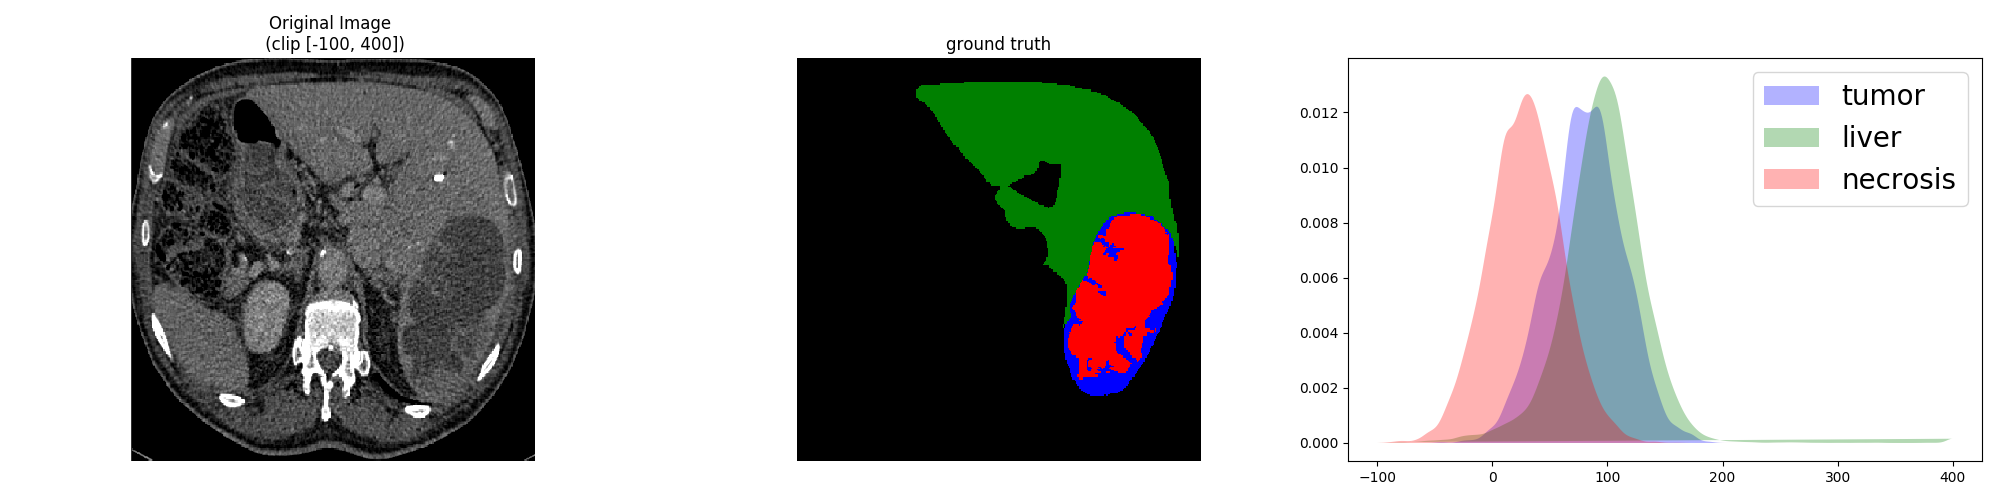
\includegraphics[width=0.7\linewidth]{images/hist}
\caption{À gauche l’image originale, au milieu les différentes zones segmentées, à droite la répartition en termes de valeur HU dans les différentes zones segmentées.}
\label{fig:hist}
\end{figure}


Les résultats obtenus par les algorithmes de segmentation sont évalués en utilisant le DICE qui est l’un des critères les plus couramment utilisés pour cette tâche.
La difficulté quant à la séparation de ces différentes classes a été prouvée par notre approche en utilisant des techniques de classification plutôt “classiques” comme la régression logistique avec un DICE moyen de 0.63 au mieux dans le cas binaire (nécrose - non nécrose dans la tumeur) et un DICE de 0.61 dans le cas multi-classes.

Nous avons choisi d’utiliser une architecture ayant déjà fait ses preuves sur des bases contenant peu de cas [49] qui est le U-Net.
Spécialement conçue pour les tâches de segmentation sémantique, ce réseau permet, à l’image des auto-encodeurs, de compresser l’information présente dans une image, mais dans le but d’aboutir ici à une carte de même taille que l’image originale où chaque pixel est représenté par sa classe d’appartenance.
L’architecture en cascade est implémentée comme dans [47]. Le foie étant automatiquement segmenté dans l’image CT originale, une nouvelle image est alors reconstruite en masquant les pixels n’appartenant pas au foie précédemment contouré. D’hypothétiques tumeurs sont recherchées et, le cas échéant, détourées par un second réseau. Enfin, le processus est répété pour la segmentation de la nécrose dans les ROIs correspondant aux tumeurs.
Les différents volumes acquis ayant été initialement recalés [50], nous avons également décidé d’analyser l’apport de l’information multiphase lors de la segmentation. Les images obtenues avant injection du produit de contraste n’apportant pas suffisamment de contraste inter-tissus, seules les phases artérielles et veineuses ont été conservées.
Nous avons adapté nos modèles de manière à soit considérer l’entrée du réseau comme une concaténation des images de la coupe z aux différents temps choisis, soit d’effectuer la segmentation sur chaque phase indépendamment puis de fusionner les résultats en queue de réseau.
Les résultats obtenus ont permis de confirmer notre hypothèse initiale, à savoir que plusieurs réseaux utilisés en cascade permettent une segmentation plus fidèle qu’un seul réseau entraîné à effectuer différentes tâches simultanément.
Des exemples de prédictions sont visibles sur la figure \ref{fig:prediction_pres}. L’information multiphase a par ailleurs permis d’améliorer les résultats notamment pour la différenciation entre la partie active et la partie nécrotique de la tumeur. Une des avancées également rendue possible par l’étude a été l’estimation automatique du taux de nécrose proche de celle effectuée par les experts. Cette valeur est un marqueur biologique important tant elle peut être liée à l’avancement de la maladie [51].
L’ensemble de ce travail a fait l’objet d’une publication [52].

\begin{figure}
\centering
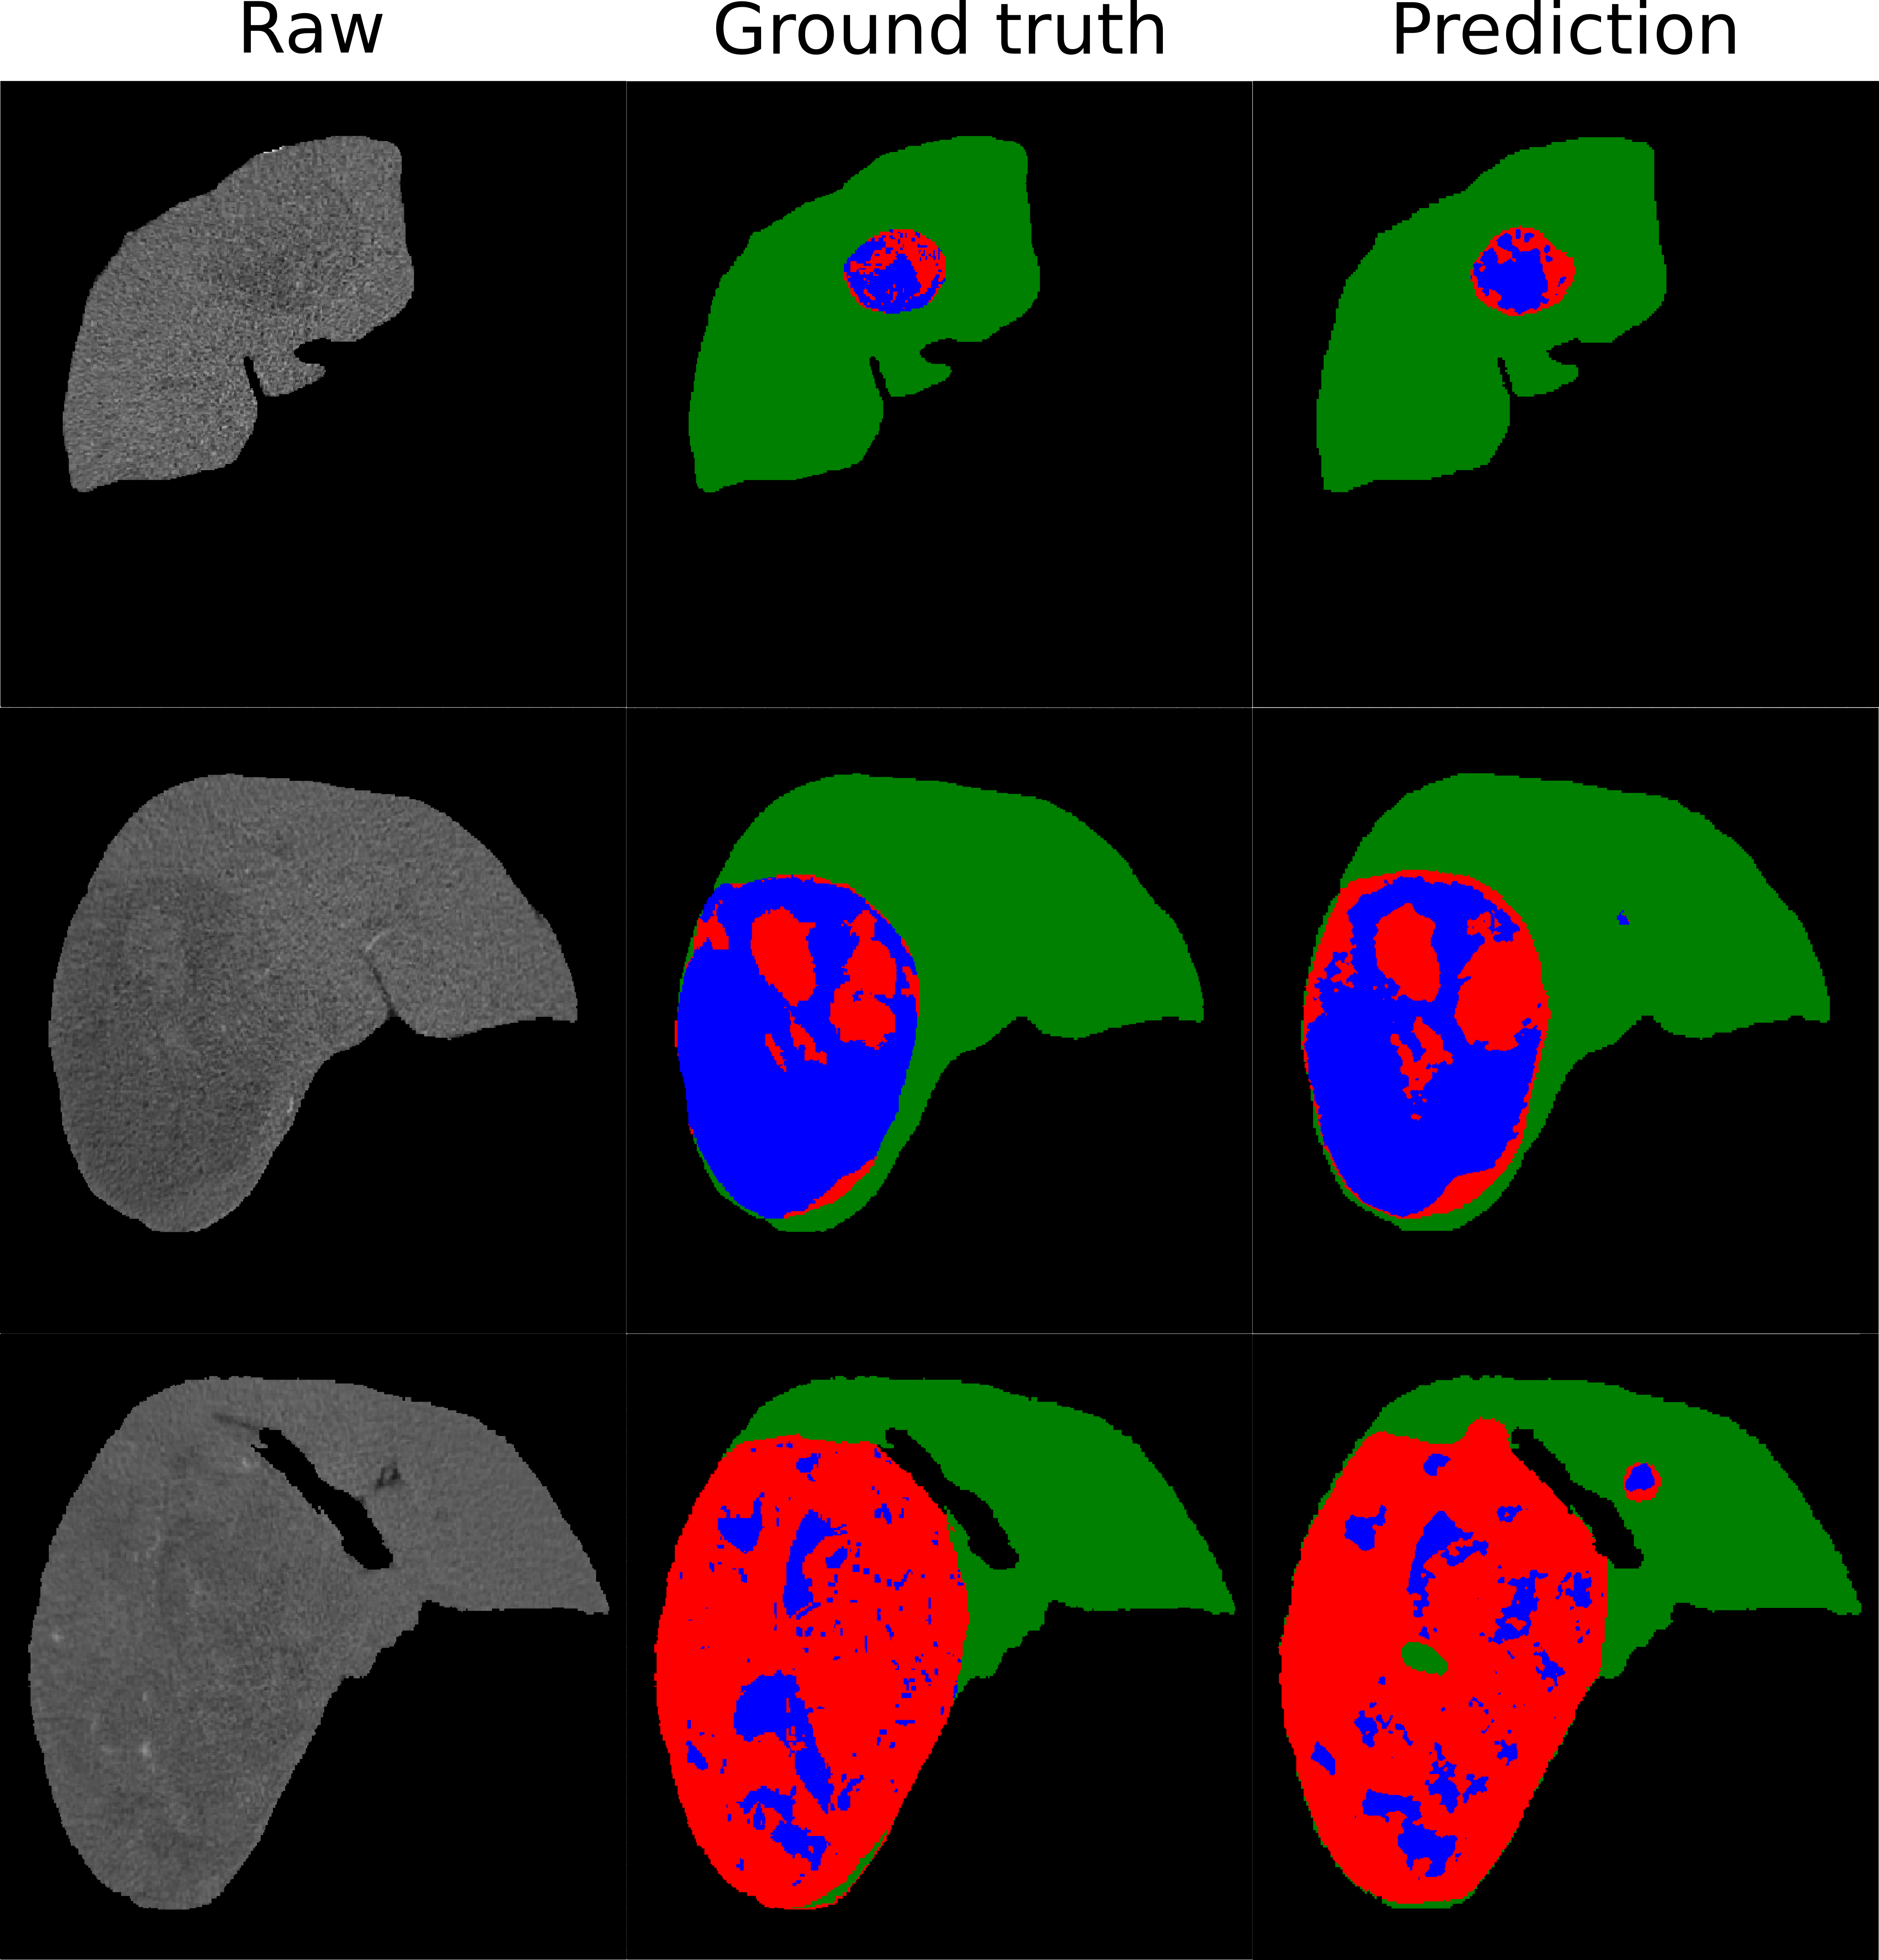
\includegraphics[width=0.7\linewidth]{images/prediction_pres}
\caption{À gauche l’image originale, au milieu la vérité terrain et à droite la prédiction obtenue après utilisation du réseau en cascade}
\label{fig:prediction_pres}
\end{figure}

Nous avons prolongé cette étude afin de proposer une architecture capable de compléter les bases de données d’images multiphase contenant peu ou aucune annotations d’experts. Pour cela, nous avons cherché à compléter 2 bases de données contenant des images CT multiphase acquises aux temps artériel et portal, que sont le base TCIA (The Cancer Imaging Archive), dont 18 patients ont été sélectionnés, et une base interne contenant 79 patients.
Les tumeurs de la base TCIA ont été segmentées par un expert, en utilisant uniquement le temps portal comme référence, tandis que la base interne présentait des segmentations pour la zone tumorale pour lesquelles le temps artériel avait été utilisé comme référence.
Afin de pouvoir créer un réseau capable de segmenter des images multiphases, l’un des pré-requis consiste à effectuer un recalage des différents volumes pour s’assurer que les structures anatomiques soient présentes à la même position spatiale d’une phase à l’autre.
Pour l’étape de recalage nous avons utilisé l’algorithme ANTS qui implémente plusieurs transformations. Dans notre cas, trois transformations ont été utilisées, à savoir une transformation rigide, suivie d’une transformation affine et d’une transformation difféomorphique. Les deux premières estiment un déplacement global de la zone à recaler tandis que la transformation difféomorphique calcule un déplacement pour chaque voxel de la région d’intérêt. Afin de permettre un recalage plus fidèle des structures que nous cherchons à analyser (foie et tumeurs) nous avons décidé d’appliquer l’algorithme en utilisant le masque du foie comme masque de recalage. Le masque du foie a été obtenu en entraînant un réseau de segmentation sémantique à partir des images de LITS. Ce réseau a permis de segmenter des images à la fois au temps artériel et au temps portal, alors qu’il avait été entraîné initialement uniquement à partir d’images monophases non étiquetées (présence d’images au temps artériel, portal et tardif).
Un réseau de segmentation des tumeurs a été entraîné à l’aide des images recalées obtenues à partir de la base interne contenant 79 patients. Chaque volume était alors associé à une annotation pour la zone du foie ainsi que des tumeurs hépatiques.
La segmentation du foie ainsi que des tumeurs pour les patients de la base TCIA a été effectuée grâce à un recalage suivi d’une délinéation par le biais des deux modèles de segmentation du foie (entraîné sur LITS) et de la tumeur (entraîné sur la base interne contenant 79 patients), tous deux associés dans une architecture en cascade.

\subsection{Deep Radiomics pour la prédiction du grade}
L’architecture en cascade choisie dans notre cas nous permet d’entraîner les différents réseaux sur des tâches spécifiques en tenant compte de la spécificité de chaque base, ce qui permet un entraînement sur le maximum de cas possible. 
Une fois les différents réseaux suffisamment robustes pour permettre une segmentation précise, nous avons implémenté une nouvelle architecture afin d’utiliser les caractéristiques extraites pour la prédiction du grade histologique.
Pour cette tâche, la seule base de données avec une vérité terrain histologique disponible était la base TCIA dont 18 cas étaient exploitables.
Les différents cas ont été séparés en deux catégories (9 patients avec grades faibles : Edmonson G1 et G2, vs 9 patients avec grades élevés : Edmonson G3) et il a été décidé, plutôt que de donner un grade à chaque patient, d’effectuer une analyse coupe à coupe. La raison principale étant que l’établissement de la vérité terrain ne se fait pas sur l’intégralité de la tumeur mais sur une inspection histologique de celle-ci, et que dans le cas du standard ES 1954, le grade sélectionné par les experts correspond au plus sévère rencontré sur la coupe histologique. Nous considérons que pour un patient donné, la zone la moins différenciée (la différenciation cellulaire va de paire avec le grade histologique) se situera près du centre de la tumeur car c’est généralement à partir de là que la maladie évolue, avec une apparition de nécrose après un certain temps. 
Le réseau de neurones choisi pour effectuer la prédiction du grade s’apparente à un algorithme de réduction de dimensionnalité où un cube de 32x32x512 descripteurs est réduit en un cube de 32x32x8 éléments avant d’effectuer la prédiction via un softmax. Les descripteurs utilisés en entrée seront ceux retenus par le modèle de segmentation sémantique multiphase des tumeurs. 
Après un entraînement en validation croisée pour permettre une meilleure reproductibilité, l’architecture composée de couches de convolutions nous a permis de prédire, dans le meilleur des cas, le bon grade pour 15 patients sur les 18, avec 74\% des coupes correctement prédites. La matrice de confusion obtenue est reportée dans le tableau \ref{tab:confusion_matrix}, avec une précision de 0.88, une spécificité de 0.78 et une sensibilité de 0.89. 


\begin{table}[!ht]
	\centering
	\caption{Matrice de confusion pour la prédiction du grade histologique par patient, LG= Low Grade, HG = High Grade}\label{tab:confusion_matrix}
	\begin{tabular}{l|l|c|c|c}
		\multicolumn{2}{c}{}&\multicolumn{2}{c}{\textbf{True grade}}&\\
		\cline{3-4}
		\multicolumn{2}{c|}{}&LG&HG&\multicolumn{1}{c}{\textit{Total}}\\
		\cline{2-4}
		\multirow{2}{*}{\textbf{Predicted grade}}& LG & \textbf{7} & 1 & 8\\
		\cline{2-4}
		& HG & 2 & \textbf{8} & 10 \\
		\cline{2-4}
		\multicolumn{1}{c}{} & \multicolumn{1}{c}{\textit{Total}} & \multicolumn{1}{c}{\textbf{9}} & \multicolumn{1}{c}{9} & \multicolumn{1}{c}{18}\\
	\end{tabular}
\end{table}


\section{Perspectives}
L’un des objectifs principaux à l’avenir serait de confirmer la capacité du réseau utilisant les caractéristiques sémantiques à pouvoir prédire le grade histologique sur d’autres patients que ceux utilisés dans notre cas. 
Un entraînement effectué sur un plus grand nombre de patients permettrait d’obtenir des résultats avec une meilleure reproductibilité. Il serait également judicieux d’inclure des patients provenant d’instituts différents afin de rendre l’ensemble du pipeline robuste aux conditions d’acquisition. Les nouvelles bases de données devraient également contenir l’information de la localisation précise de la nécrose afin de pouvoir l’incorporer dans le processus de prédiction du grade. Cependant, la segmentation, faite par un ou plusieurs experts, de la partie nécrotique de la tumeur s’effectue dans la plupart des cas sur une phase unique, ce qui ne rend pas compte de l’évolution temporelle de celle-ci. Il serait donc préférable de constituer une base de données avec des zones nécrotiques segmentées par différents experts et sur l’ensemble des phases disponibles, et ceci afin de pouvoir implémenter un réseau neuronal capable d’extraire automatiquement les caractéristiques propres à cette région. 
L’extraction des caractéristiques d’images nécessaires à la prédiction du grade se faisant dans notre cas à partir d’un réseau effectuant la segmentation sémantique, il serait également judicieux d’améliorer les performances obtenus par celui-ci, notamment via l’inclusion de convolutions entièrement 3D, ce qui n’est pas encore le cas dans notre travail. Nous avons en effet démontré que l’ajout de coupes adjacentes permettait d’améliorer légèrement la précision de la segmentation, cependant le problème de l’espacement inter-coupe ainsi que le coût en temps de calcul ne nous a pas encore permis d’implémenter une architecture avec des couches de convolution 3D. Cette amélioration nous permettrait de mieux appréhender la structure spatiale de la tumeur, ce qui rendrait également possible une étude locale de la différentiation. Résoudre le problème de la 3D permettrait également de construire une architecture de prédiction du grade dont l 'intégralité de l’information volumétrique serait considérée, comme avec un LSTM, plutôt que d’effectuer une prédiction coupe à coupe comme c’est le cas dans nos expériences.
Enfin, la grande nouveauté apportée par notre étude est l’incorporation de l’information multiphase, lors de la segmentation sémantique ainsi que lors la prédiction du grade histologique. Nous avons en effet démontré que l’utilisation d’images obtenues à différents moments après injection d’un produit de contraste permettait d’améliorer la détection et la délinéation de lésions tumorales. L’acquisition d’images tomographiques du foie à des fins de diagnostic s’effectue la plupart du temps en suivant un modèle triphasique, mais aucun standard n’existe quant à la définition précise des temps auxquels les différentes acquisitions doivent se faire. En l’absence de directives précises, il serait nécessaire de trouver un moyen qui puisse automatiquement déterminer la durée précise entre l’administration du produit de contraste et l’acquisition d’une image donnée. Des pistes ont été explorées dans notre cas comme la spécification d’histogramme, mais la mise en place d’une telle technique nécessite une base de données avec un nombre élevé de patients pour être suffisamment robuste aux cas particuliers. D’autres solutions pourraient être envisagées comme la constitution d’une base contenant des images avec l’information précise de la durée entre l’injection et l’acquisition, ainsi que d’autres informations expérimentales comme la vitesse d’injection, ou encore le flux sanguin.


\newpage
%\bibliographystyle{unsrt}
\printbibliography[heading=bibintoc]

\end{document}